% Niveau :      PCSI *
% Discipline :  Chimie Orga
% Mots clés :   Infrarouge

\begin{exercise}{Spectre infrarouge de l'eau}{2}{PCSI}
{Chimie organique I,Spectroscopie,Infrarouge}{bermu}

\begin{questions}
\questioncours Spectroscopie infrarouge
\begin{itemize}
    \item principe physique ;
    \item exemple d'une molécule diatomique simple ;
    \item paramètres influençant la fréquence de résonance et la largeur spectrale des raies ;
\end{itemize}

\uplevel{On considère désormais la molécule d'eau $\mathrm{H_2O}$.}

\question Donnez sa géométrie selon la théorie VSEPR.

\question Quels sont les différents modes de vibration de la molécule d'eau ? Les illustrer par un schéma.

\begin{EnvUplevel}
    On donne ci-dessous les spectres IR de l'eau $\mathrm{H_2O}$ et de l'eau ‘lourde’ $\mathrm{D_2O}$.
    
    \begin{figure}[H]
        \centering
        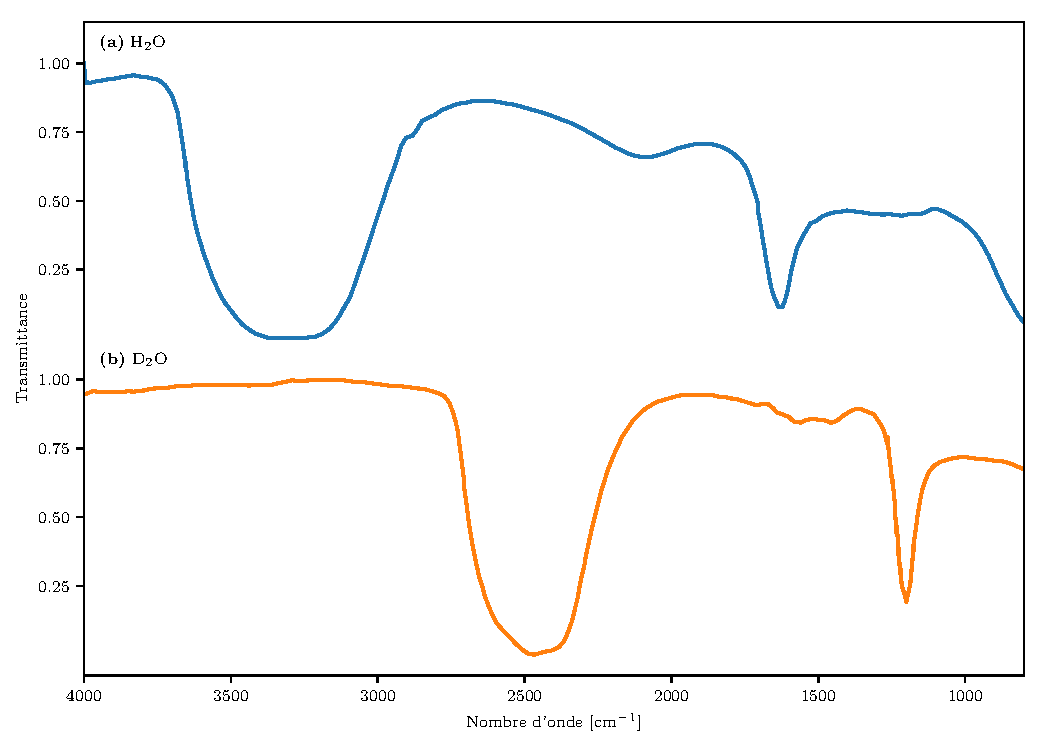
\includegraphics[width=\linewidth]{chimiePC/orga/H2OD2O.pdf}\vspace{-1em}
        \caption{Spectres infrarouges de l'eau et de l'eau lourde.}
    \end{figure}
\end{EnvUplevel}

\question Interprétez quantitativement les spectres ci-dessous à l'aide de la question de cours.

\question A quoi est dû le fort élargissement de la bande 3500 cm$^{-1}$ (2500 cm$^{-1}$ pour $\mathrm{D_2O}$) ?
\end{questions}
\end{exercise}